
\section{\textcolor{Navy}{Extended Visual Analysis}}
\subsection{\textcolor{Teal}{Attack mechanism and wealth accounting}}
The figures in this section explain the same model used in the formal analysis.
The diagrams show transitions and assumptions; the measurement plots reuse the
saved experiment dataset. No additional solver experiment is implied.

\begin{figure}[!ht]\centering
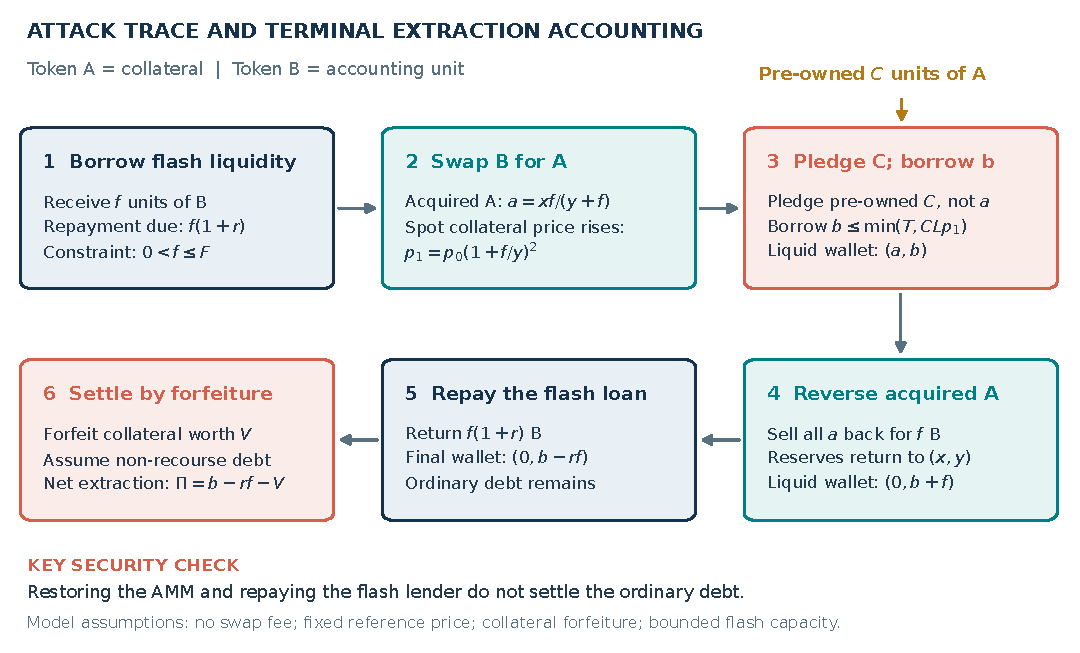
\includegraphics[width=0.97\textwidth]{figures/color-attack-flow.pdf}
\caption{Illustrated core attack schedule. The pre-owned collateral is separate
from the AMM tokens acquired during manipulation. Collateral forfeiture is the
settlement assumption that turns the residual lending debt into extraction.}
\label{fig:attack-visual}\end{figure}

\begin{table}[!ht]\centering
\caption{Constructed optimal example: attacker wallet and protocol state.}
\begin{tabular}{lrrrrl}\toprule
\textcolor{Navy}{Stage} & \textcolor{Navy}{Wallet $A$} & \textcolor{Navy}{Wallet $B$} & \textcolor{Navy}{AMM $x$} & \textcolor{Navy}{AMM $y$} & \textcolor{Navy}{Other obligation/state}\\\midrule
Initial & 100 & 0 & 1000 & 1000 & No debt\\
Flash acquisition & 100 & 1000 & 1000 & 1000 & Flash due: 1000.9 $B$\\
Manipulating swap & 600 & 0 & 500 & 2000 & Spot price: 4 $B/A$\\
Pledge and borrow & 500 & 300 & 500 & 2000 & Custody: 100 $A$; debt: 300 $B$\\
Reverse swap & 0 & 1300 & 1000 & 1000 & Ordinary debt persists\\
Repay flash loan & 0 & 299.1 & 1000 & 1000 & Flash obligation discharged\\
Forfeit collateral & 0 & 299.1 & 1000 & 1000 & Net extraction: 199.1 $B$\\
\bottomrule\end{tabular}\label{tab:ledger}\end{table}

The ledger uses $f=1000$, $C=100$, $L=0.75$, $r=0.0009$ and $T=400$.
The final wallet is 299.1 units of $B$, but initial wealth was worth 100 units.
Consequently, net extraction is 199.1 rather than 299.1. The lending protocol
holds collateral with reference value 100 against debt 300. Under the stipulated
settlement, the lender's 200-unit shortfall is split between attacker extraction
of 199.1 and the flash lender's fee of 0.9. No token conservation law is violated.

\takeaway{\textbf{Security interpretation.} Restoring AMM balances and repaying the
flash lender do not restore the attached lender's collateral coverage. Economic
safety must be checked across the whole modeled transaction.}

\clearpage
\subsection{\textcolor{Teal}{How a model becomes a verification result}}
The solver searches for any feasible execution with positive extraction. The
analytical calculation provides a separate criterion for the fixed core model,
while exact replay checks that a returned rational witness obeys its transitions.

\begin{figure}[!ht]\centering
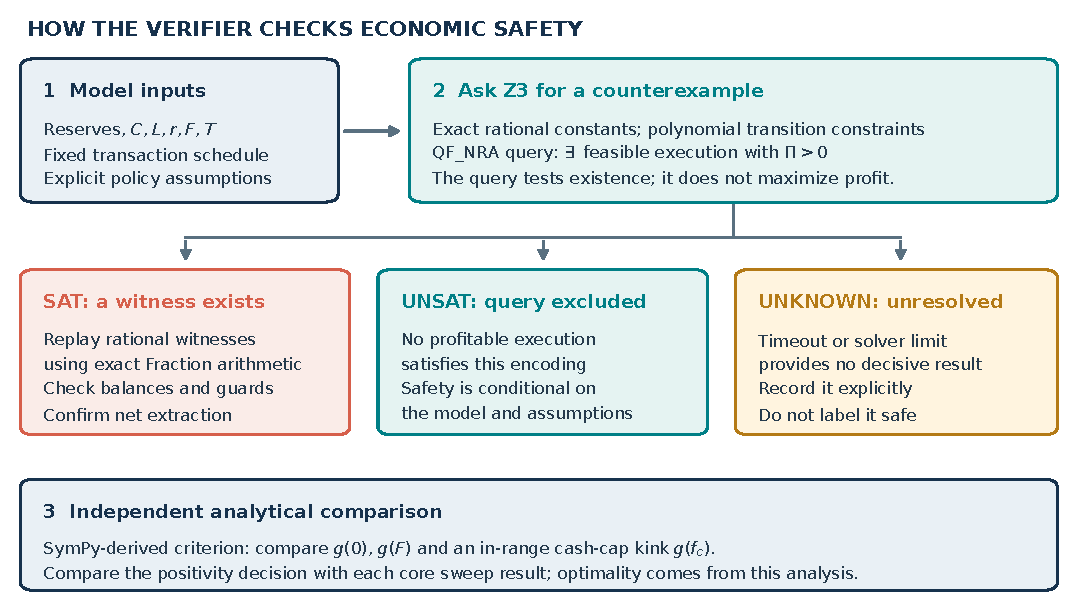
\includegraphics[width=0.97\textwidth]{figures/color-verification-pipeline.pdf}
\caption{Verification workflow. SAT, UNSAT and UNKNOWN carry different meanings.
The analytical criterion is specific to the capped core profit function. Exact
replay checks a witness; it is not an independently checked UNSAT certificate.}
\end{figure}

\begin{table}[!ht]\centering
\caption{Defenses, sufficient conditions, and limits of the evidence.}
\begin{tabular}{p{0.20\textwidth}p{0.35\textwidth}p{0.35\textwidth}}\toprule
\textcolor{Navy}{Defense} & \textcolor{Navy}{Required model condition} & \textcolor{Navy}{What remains to justify in practice}\\\midrule
Bounded oracle & $p_{\rm oracle}\leq p_0(1+\epsilon)$ and $L(1+\epsilon)\leq1$ & Show the concrete oracle enforces the assumed bound.\\
Rational dynamic LTV & $L(f)=L_0/(1+f/y)^2$, with $L_0<1$ & Establish how the relevant distortion is measured and enforced.\\
Sufficient reserve depth & $y\geq y_{\rm safe}$ for fixed $V,L,r,F,p_0$ & Justify collateral value, capacity and price assumptions.\\
Corrected vault minting & Use the proxy's true pre-deposit assets for share issuance & Verify the deployed vault's valuation and settlement rules.\\
Donation health guard & Post-donation collateral must cover debt at the given threshold & Model liquidation and all other routes to unhealthy debt.\\
\bottomrule\end{tabular}\end{table}

\takeaway{\textbf{Reading the labels.} SAT means the encoded target is reachable.
UNSAT excludes that target under the model's assumptions. UNKNOWN leaves the
question unresolved. A label is meaningful only together with the property checked.}

\clearpage
\subsection{\textcolor{Teal}{Measured decisions and solving-time distribution}}
Figure~\ref{fig:measured} separates the number of distinct parameter settings
from the number of solver calls. It also exposes the variation hidden by a
single median. Colors identify decisions; horizontal navy marks show medians.

\begin{figure}[!ht]\centering
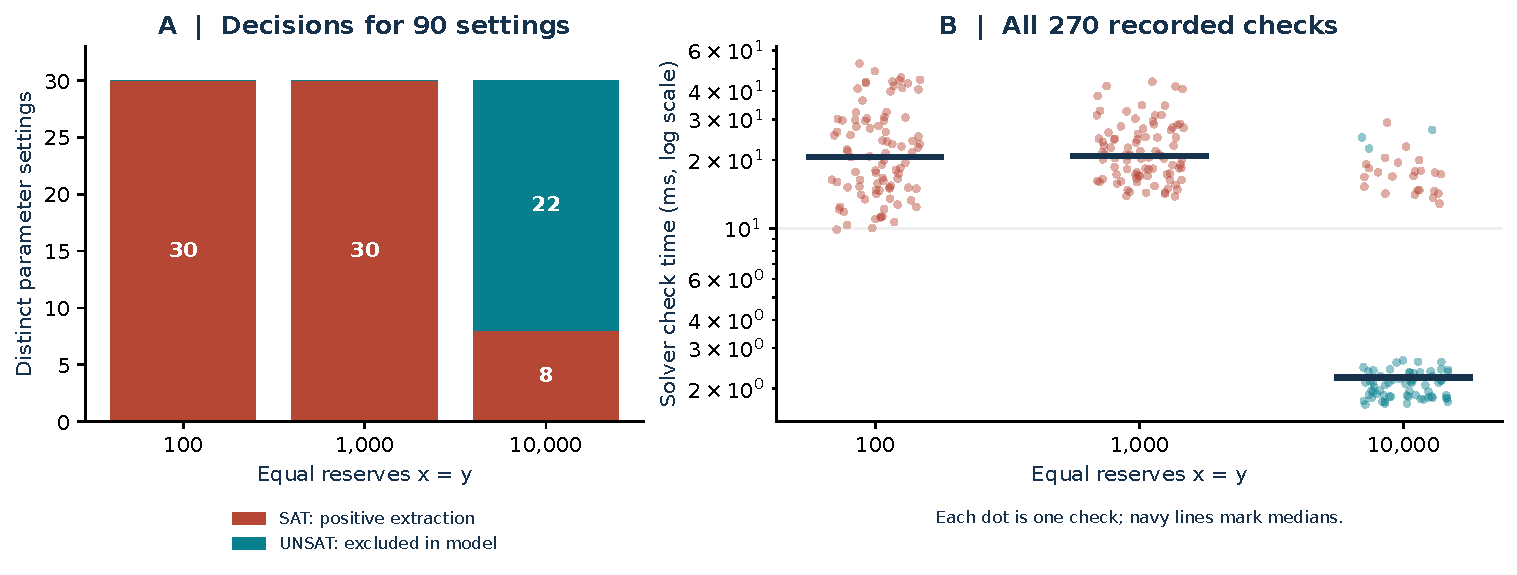
\includegraphics[width=0.98\textwidth]{figures/color-measured-overview.pdf}
\caption{Left: decisions for the 90 distinct settings. Right: solver-check time
for all 270 recorded calls on a logarithmic axis. There were no UNKNOWN results.
Each reserve group contains 30 settings and 90 calls.}
\label{fig:measured}\end{figure}

\begin{table}[!ht]\centering
\caption{Decision counts by distinct setting and descriptive timing statistics.}
\begin{tabular}{rrrrrrr}\toprule
\textcolor{Navy}{$x=y$} & \textcolor{Navy}{SAT settings} & \textcolor{Navy}{UNSAT settings} & \textcolor{Navy}{Min. ms} & \textcolor{Navy}{Median ms} & \textcolor{Navy}{P95 ms} & \textcolor{Navy}{Max. ms}\\\midrule
100 & 30 & 0 & 9.894 & 20.606 & 44.127 & 52.619\\
1,000 & 30 & 0 & 13.823 & 20.785 & 36.477 & 43.826\\
10,000 & 8 & 22 & 1.701 & 2.233 & 21.472 & 29.053\\
\bottomrule\end{tabular}\end{table}
The timing columns use all 90 calls at each reserve depth. P95 is the 95th
percentile with linear interpolation. It describes this sample; it is not a
confidence bound. Constraint construction and witness replay are outside these times.

\begin{table}[!ht]\centering
\caption{Experimental grid and counting rules.}
\begin{tabular}{lll}\toprule
\textcolor{Navy}{Dimension} & \textcolor{Navy}{Values} & \textcolor{Navy}{Count}\\\midrule
Equal reserve depth & 100; 1000; 10000 & 3\\
Loan-to-value limit & 0.50 to 0.95 in steps of 0.05 & 10\\
Flash fee rate & 0.09\%; 0.15\%; 0.30\% & 3\\
Fixed economic inputs & $C=100$, $F=1000$, $T=400$, $p_0=1$ & Constant\\
Distinct settings & $3\times10\times3$ & 90\\
Repeated solver calls & 3 per setting & 270\\
\bottomrule\end{tabular}\end{table}

\takeaway{\textbf{Observed pattern.} The deepest pool has 22 UNSAT settings out of
30; the other two depths have none in this grid. These proportions describe
selected synthetic settings, not the probability that a real protocol is attacked.}

\clearpage
\subsection{\textcolor{Teal}{Decision boundary and analytical profit curves}}
\begin{figure}[!ht]\centering
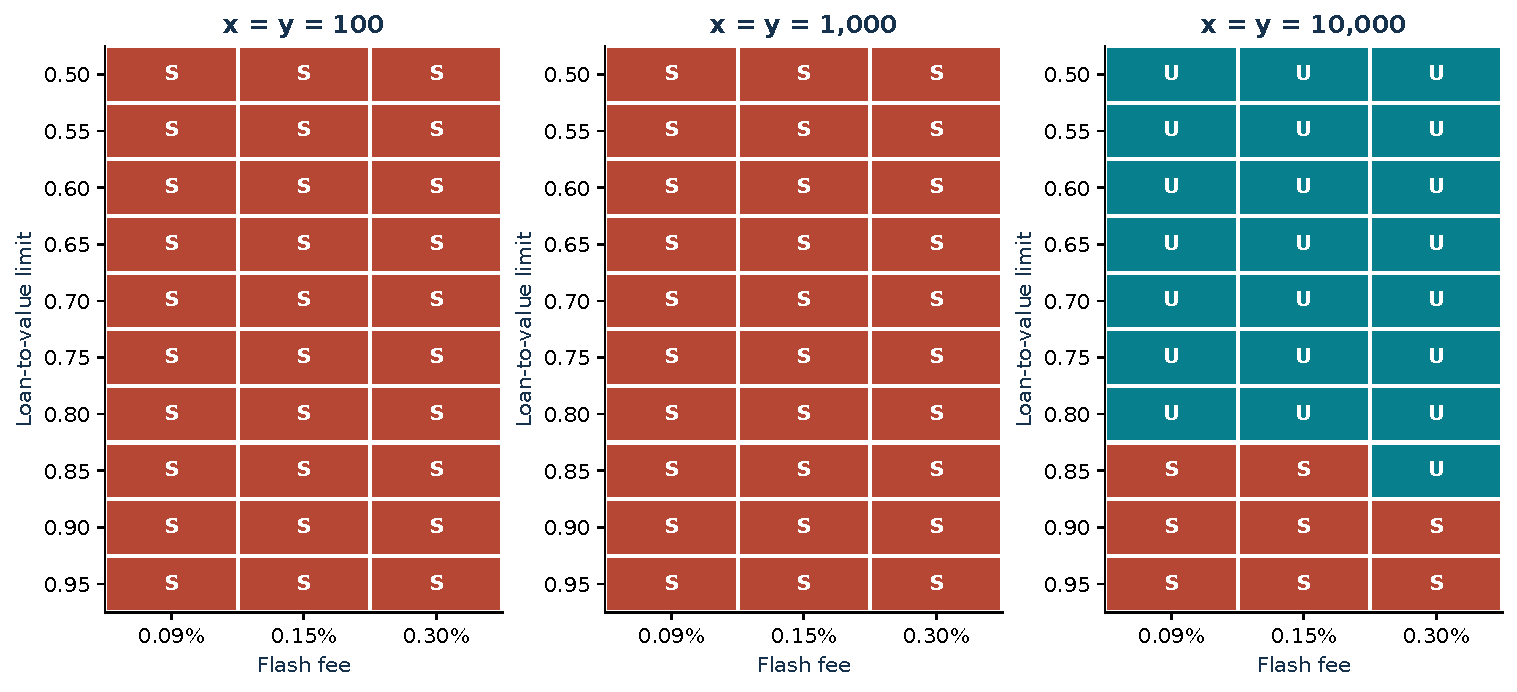
\includegraphics[width=0.98\textwidth]{figures/color-decision-map.pdf}
\caption{Recorded decision map. S (coral) denotes SAT and U (teal) denotes UNSAT.
Each cell is one parameter setting; all three repeats agree. Lower LTV and
greater reserve depth can exclude extraction within this fixed grid.}
\end{figure}

\begin{figure}[!ht]\centering
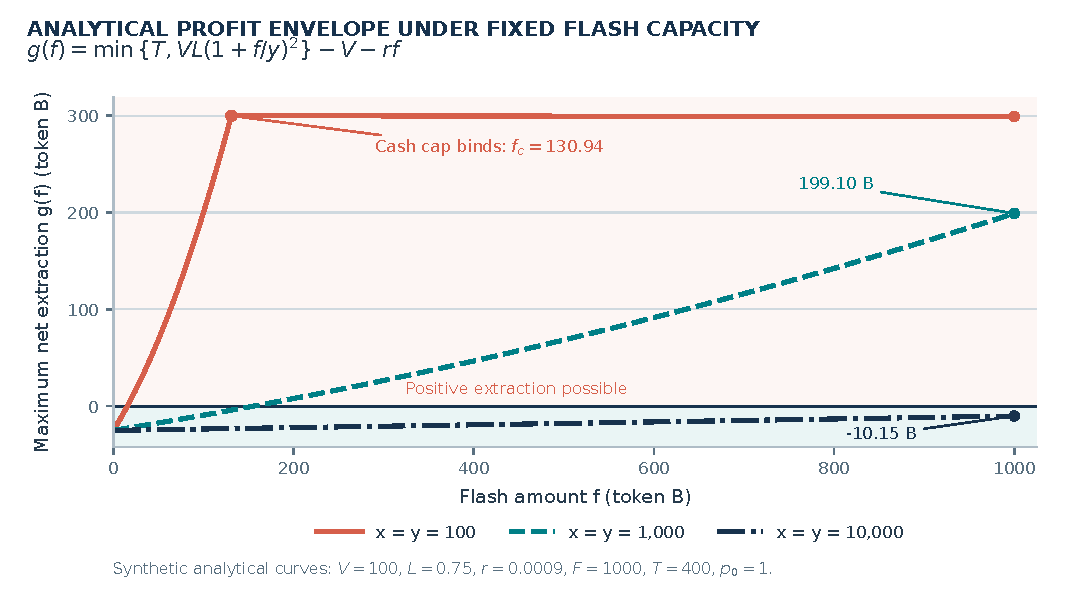
\includegraphics[width=0.92\textwidth]{figures/color-profit-curves.pdf}
\caption{Analytical illustration of $g(f)$, using $V=100$, $L=0.75$, $r=0.0009$,
$T=400$, $F=1000$ and the indicated reserve depth. This evaluates the derived
formula; the plotted points are not new solver measurements. The zero line
separates positive extraction from nonpositive net outcomes.}
\end{figure}

The shallow pool reaches the cash cap within the allowed interval. Beyond that
kink the marginal effect of another unit of flash liquidity is the negative
flash fee. At the baseline depth of 1000 the endpoint $f=1000$ yields 199.1.
At depth 10000 the entire curve stays below zero for the displayed LTV and fee.
The limit $f=0$ is included to visualize the analytical endpoint; a flash attack
in the core query requires $f>0$.
